\chapter{Testes e observações}\label{sec:resultados}

\section{Coleta dos dados}\label{sec:coleta}

O dados foram coletados de cinco máquinas do ambiente de compilação do
projeto Mandriva Linux entre os dias 15 de março de 2011 e 11 de abril de
2011, com medidas de uso tempo de uso de CPU sendo realizadas a cada 30
segundos, resultando num total de 80~200 valores para cada máquina.

Todas as máquinas possuem 4 CPUs e \emph{clock} de 2~800MHz. As máquinas n2,
n3 e n4 são utilizadas exclusivamente para execução de software para
arquitetura i686 (32 bits,) enquanto que n6 e seggie são utilizadas para
execução e compilção de software em arquitetura AMD64 (64 bits.)

\section{Caracterização}

Mesmo estas máquinas fazendo parte de um ambiente de compilação que é
utilizado diariamente para compilar vários pacotes de software do projeto
Mandriva Linux, 45\% dos valores de uso de CPU lidos foram 0\%, ou seja,
as máquinas estiveram ociosas durante 45\% do tempo durante os 27 dias de
coleta. A figura \ref{fig:prehistn4} mostra a distribuição para uma das
máquinas do ambiente. Os histogramas das outras máquinas estão no apêndice
\ref{chap:histogramas}, a partir da página \pageref{chap:histogramas}.

\begin{figure}[htp]
\centering
\includegraphics{src/test-data/workload/histograma-n4.pdf}
\figinfo{Distribuição dos valores de uso de CPU da máquina n4}
\label{fig:prehistn4}
\end{figure}


A figura~\ref{fig:predispn4} mostra a dispersão dos valores de CPU durante
todo o período de observação, enquanto que a figura~\ref{fig:disp4hn4}
mostra o o comportamento durante um período de quatro horas, aonde é
possível observar mais claramente cada ponto observado. Nota-se que a
transição entre os valores é pouco suave. O valor do desvio padrão para
cada máquina está disposto no quadro \ref{quadro:desviopadrao}.

\begin{table}[htp]
\centering
\hspace{-2cm} % FIXME arrumar no template
\quadro{Média e desvio padrão das máquinas observadas}\label{quadro:desviopadrao}
\begin{tabular}{| c | c | c | c |}
\hline
Máquina & Média & Desvio padrão \\
\hline
n2 	& 	24,5623722901 & 34,45394416 \\
n3 	& 	6,83392723648 & 18,5214665282 \\
n4 	& 	27,7236937184 & 32,1217945295 \\
n6 	& 	35,1048768939 & 37,8408009198 \\
seggie 	&	19,9159114989 & 32,068825708 \\
\hline
\end{tabular}
\end{table}

\begin{figure}
\centering
\includegraphics[width=0.7\textwidth]{src/test-data/workload/dispersion-n4.png}
\figinfo{Representação dos valores de uso de CPU da máquina n4}
\label{fig:predispn4}
\end{figure}

Nesta mesma figura~\ref{fig:disp4hn4} é possível observar o ciclo de vida
de uma tarefa de compilação de um pacote de software. A partir do ponto 150
nota-se um crescimento moderado no uso de CPU, que pode ser associado ao
estágio de preparação que é executado antes da compilação em si. Este
estágio executa a descompressão dos códigos-fonte que serão compilados,
geralmente usando os softwares gzip\footnote{http://www.gzip.org} e
bzip2\footnote{http://bzip2.org}. Tal descompressão é uma tarefa faz uso
intenso de leitura e escrita de disco e também de CPU, porém estas
ferramentas fazem uso apenas de uma CPU, resultando em leituras de CPU em
torno de 25\%.

Após o estágio de preparação o software é compilado. A maioria dos
códigos-fonte é preparada para compilar código paralelamente, permitindo
assim fazer uso de todas as CPUs disponíveis, chegando aos 100\% de
utilização. Finalmente, quando a tarefa de compilação é concluída os
binários gerados são comprimidos em um arquivo, resultando novamente no uso
moderado de CPU.

\begin{figure}[htp]
\centering
\includegraphics[width=0.7\textwidth]{src/test-data/workload/dispersion-4h-n4.png}
\figinfo{Representação dos valores de uso de CPU da máquina n4 durante um
período de 4 horas}
\label{fig:disp4hn4}
\end{figure}

É possível observar também na figura \ref{fig:predispn4}, e também nas
figuras \ref{fig:appdispn2}, \ref{fig:appdispn6} e \ref{fig:appdispseggie} no
apêndice, que existe um período de intenso uso de CPU em torno do ponto
30~000. Isso deve-se a uma extensa tarefa de recompilação que durou
aproximadamente três dias e utilizou várias máquinas do ambiente de
compilação.

\section{Predição}

O primeiro passo ao avaliar as técnicas de predição foi ajustar os
parâmetros que eram utilizados pelas mesmas para o domínio de dados que é
utilizado neste projeto. Para o caso de $k$-NN, o parâmetro investigado é o
número de vizinhos ($k$), e no caso de SVM, $C$ e $\sigma$, descritos a
partir da página \pageref{sec:margenssuaves}. Além disso, há outros dois
parâmetros que são específicos a este projeto e são relacionados à etapa de
predição: o tamanho da janela utilizada para treinamento e o tamanho da
janela utilizada para definir o uso de CPU futuro.

Decidiu-se por adotar a seguinte estratégia ao escolher os parâmetros:
primeiro foram utilizados para os parâmetros de valores futuros e tamanho
de janela valores que podem ser considerados “ideais” para o problema deste
projeto. Tendo esses parâmetros fixos, foi possível fazer a busca pelos
melhores parâmetros para $k$-NN e SVM. Então, tendo os parâmetros
específicos de cada técnica, foram feitos testes com diferentes tamanhos de
janela para treinamento e futuro.

% me dei conta agora que a definição de “futuro” deveria estar associada à
% influência que realmente o valor vai ter no vetor de características

O tamanho de janela considerado ideal para este projeto foi 10, ou seja,
representa um horizonte de 5 minutos. Este período de tempo é suficiente
para incluir o tempo de migração das máquinas virtuais (abordado a seguir.)

Para os testes de $k$ de $k$-NN, foi utilizado um programa escrito em
\emph{shell script} que executa a etapa de treinamento e predição para
valores de $k$ que vão de 2 até 20 e também para 30, 40, 50, 75, 100 e 150
vizinhos. O script utilizado está no apêndice \ref{chap:programasteste}. A
figura \ref{fig:knnn4} mostra a taxa de acerto de acordo com o valor de $k$
para a máquina n4.

\begin{figure}[htp]
\centering
\includegraphics[width=0.8\textwidth]{src/test-data/classification/knn-n4.pdf}
\figinfo{Distribuição dos valores de uso de CPU da máquina n4}
\label{fig:knnn4}
\end{figure}

Para o caso de SVM, foram utilizadas os parâmetros sugeridos por
\citeonline{hsu2003practical}, com valores de $C$ indo de $2^{-5}$ até
$2^9$ e $\sigma$ de $^{-15}$ até $2^{3}$.  Após
isso, foi executada mais uma rodada de testes, desta vez utilizando uma
faixa de valores mais curta, indo de 0,3125 até 2, tando para $C$ quanto
para $\sigma$. A figura \ref{fig:svmn4} apresenta o desempenho desses parâmetros
para utilizando dados da máquina n4. O script utilizado para testes está no
apêndice \ref{chap:programasteste}.

%%% XXX XXX XXX CROSS VALIDATION!!!
%%% XXX figura de parâmetros da SVM aqui!

\begin{figure}[htp]
\centering
\includegraphics[width=0.8\textwidth]{src/test-data/classification/svm-n4-finer.pdf}
\figinfo{Espaço de busca de $C$ e $\sigma$ para SVM}
\label{fig:svmn4}
\end{figure}

Finalmente, foram feitos os testes utilizando diferentes tamanhos de janela
para trainamento e valores futuros. A figura \ref{fig:svmwindowfuturen4} apresenta o
espaço de busca e o desempenho utilizando dados da máquina n4.

\begin{figure}[htp]
\centering
\includegraphics[width=0.8\textwidth]{src/test-data/classification/svm-n4-window-future.pdf}
\figinfo{Espaço de busca de tamanhos de janela para classificação e futuro para
SVM}
\label{fig:svmwindowfuturen4}
\end{figure}

O quadro \ref{quadro:clageral} apresenta o desempenho observado para cada
máquina utilizando os parâmetros escolhidos para uso na etapa de consolidação.

\begin{table}[htp]
\centering
\hspace{-2cm} % FIXME arrumar no template
\quadro{Desempenho de classificação para SVM e $k$-NN}\label{quadro:clageral}
\begin{tabular}{| l | c | c | c | c | c | c |}
\hline
\multirow{2}{*}{Técnica} & \multicolumn{6}{c|}{Máquina treinada} \\
\cline{2-7}
		& n2      & n3       & n4      	 & n6        & seggie  	 & média   \\
\hline
SVM     	& 99,32\%  & 99,78\% &   99,68\% &   99,34\% &   99,20\% & 99,46\% \\
\hline
$k$-NN  	& 97,22\%  & 99,04\% &   97,60\% &   96,88\% &   95,89\% & 97,33\% \\
\hline
\end{tabular}
\end{table}

\subsection{Classificação cruzada}

\begin{table}[htp]
\centering
\hspace{-2cm} % FIXME arrumar no template
\quadro{Desempenho de classificação cruzada, usando SVM}\label{quadro:clacruzada}
\begin{tabular}{| l | c | c | c | c | c | c |}
\hline
\multirow{2}{*}{Máq. classificada} & \multicolumn{6}{c|}{Máquina treinada} \\
\cline{2-7}
		& n2      & n3       & n4      	 & n6        & seggie  	 & média   \\
\hline
n2      	& 99,39\%  & 98,59\% &   99,51\% &   96,10\% &   96,05\% & 97,93\% \\
n3      	& 99,82\%  & 99,78\% &   99,91\% &   99,09\% &   99,08\% & 99,54\% \\
n4      	& 99,39\%  & 99,11\% &   99,68\% &   98,50\% &   98,52\% & 99,04\% \\
seggie  	& 98,73\%  & 98,06\% &   99,09\% &   99,20\% &   99,38\% & 98,89\% \\
n6      	& 99,13\%  & 98,30\% &   99,27\% &   99,34\% &   99,36\% & 99,08\% \\
\hline
\end{tabular}
\end{table}

Para o caso de máquinas desconhecidas, como descrito na seção
\ref{sec:maquinasdesconhecidas}, o software tentará recorrer ao histórico
de uma máquina especial, chamada \emph{generic}. Assim, para o grupo de
máquinas estudado neste projeto, foi feito um teste em que todas as
máquinas tiveram seus históricos preditos por todas as outras máquinas, de
maneira a identificar qual delas tem melhor capacidade de generalização
para o ambiente observado, e assim cumprir o papel de \emph{generic}. No quadro
\ref{quadro:clacruzada}, que apresenta os desempenhos obtidos, é possível
observar que a máquina n4 possui o melhor desempenho de classificação.

\section{Testes de virtualização}

\subsection{Ambiente de testes}

O ambiente utilizado para testes de virtualização é composto por três máquinas
hospedeiras, a máquina tcc159 tendo processador Intel Core i3 550, \emph{clock}
de 3GHz e 4 gigabytes de memória RAM, e as outras duas máquinas, lviv e tcc158,
com processador Intel Pentium Dual-Core, \emph{clock} de 3GHz e 4 gigabytes de
memória RAM. A rede de dados utilizada para conectar estas máquinas era do tipo
100BASE-TX, que pode transmitir dados a 100 megabits por
segundo\footnote{http://standards.ieee.org/about/get/802/802.3.html}.

%% FIXME descrever o uso de NFS, bridge e essas coisas!!!!!

As máquinas virtuais eram instalações mínimas de Mandriva Linux, com imagens de
disco ocupando 1 gigabyte, emulando máquinas com processador i686 e 128
megabytes de RAM.

\subsection{Migração}

Para conhecer o tempo esperado de uma migração entre uma máquina hospedeira e
outra, foram feitas 50 migrações de máquinas virtuais, em ambos os sentidos.
Observou-se que o tempo médio de migração foi de 8,9 segundos, com desvio padrão
de 0,8 segundos.

Deve-se levar em consideração que as máquinas virtuais utilizadas para este e
outros testes no trabalho têm apenas 128MB de memória RAM, o que é uma
quantidade de memória muito pequena para os padrões de uso atuais. Porém,
espera-se que em casos aonde as máquinas virtuais tenham mais memória, seja
utilizada uma rede do tipo \emph{gigabit} (1000BASE-TX), que permite ter taxas
de transmissão pelo menos dez vezes mais rápidas.

\subsection{Simulação de carga}\label{sec:loadsim}

Para que seja possível avaliar o produto final deste projeto, ou seja, a
consolidação de máquinas virtuais, foi necessário avaliar também a técnica
utilizada para reproduzir o comportamento de uso de CPU de máquinas virtuais de
acordo com um histórico de outra máquina, descrita na seção \ref{sec:desemp}. O
teste durou uma hora e utilizou um intervalo de 10 segundos entre cada valor de
carga.

Para tal, foi implementado um programa em linguagem Python que utiliza \emph{busy
loops} para simular a carga de CPU. Seu código fonte está no apêndice, página
\pageref{fig:progsimload}.

A figura \ref{fig:simworkload} apresenta o uso de CPU medido da máquina virtual
sobreposto com o histórico que foi obtido da máquina n4. Pode-ser observar que,
mesmo com alguns \emph{outliers}, a maioria dos valores foi corretamente
simulada.

\begin{figure}
\centering
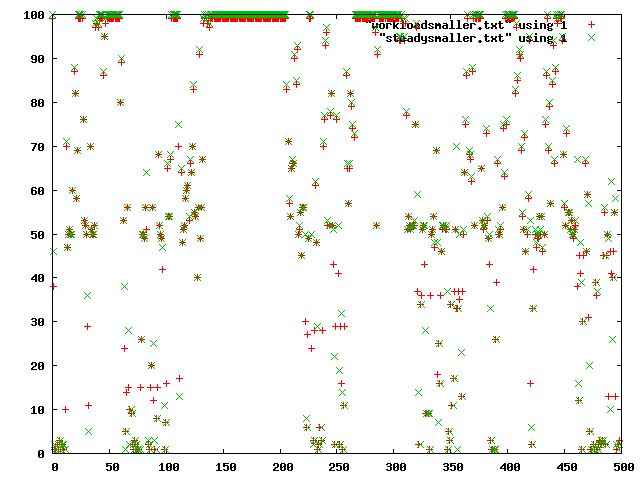
\includegraphics[width=0.7\textwidth]{src/test-data/checking-load-simulator/load-simulator-n4.png}
\figinfo{Sobreposição entre histórico de uso de CPU e observado em MV}
\label{fig:simworkload}
\end{figure}

\section{Consolidação}

Para a etapa de consolidação, foram feitos dois tipos de testes. Um simulado, em
que históricos de máquinas são utilizados para fornecer informações de uso de
CPU ao software de consolidação que faz parte deste projeto. O outro tipo de
teste consiste em simular a carga em máquinas virtuais reais, utilizando a
biblioteca \libvirt{} para acessar as informações de uso de CPU.

\subsection{Carga simulada}

Para o teste de carga simulada, foram utilizados históricos de carga de CPU que
foram coletados das máquinas observadas, descritas na seção \ref{sec:coleta}.
Neste ambiente simulado foram adicionados três hospedeiros com 4 CPUs cada. Os
testes foram executados na máquina tcc159. O quadro \ref{quadro:simula0}
apresenta os resultados obtidos para o período de 24 horas, ao passo que o
quadro \ref{quadro:simula1} apresenta o desempenho para 7 dias.

\begin{table}[htp]
\centering
\hspace{-2cm} % FIXME arrumar no template
\quadro{Resultados do teste de consolidação simulado para um dia}\label{quadro:simula0}
\begin{tabular}{| c | c | c | c | c | c |}
\hline
Técnica & Migrações & host0  & host1   & host2 & Dur. Simulação \\
\hline
$k$-NN 	& 98        & 24h    & 3:24:30 & 0h    & 12:31  \\
\hline
SVM 	& 120       & 24h    & 3:39:00 & 0h    & 02:23  \\
\hline
\end{tabular}
\end{table}

\begin{table}[htp]
\centering
\hspace{-2cm} % FIXME arrumar no template
\quadro{Resultados do teste de consolidação para sete dias}\label{quadro:simula1}
\begin{tabular}{| c | c | c | c | c | c |}
\hline
Técnica & Migrações & host0  & host1    & host2       & Dur. Simulação \\
\hline
$k$-NN 	& 510        & 168h  & 13:00    & 26:14:30    & 1:50:17  \\
\hline
SVM 	& 550        & 168h  & 13:30 	& 27:01:30    & 31:46  \\
\hline
\end{tabular}
\end{table}

É possível observar na figura \ref{fig:svmhosts} que durante toda a simulação no
máximo dois hospedeiros foram utilizados ao mesmo tempo. Além disso, o
comportamento do escalonador foi praticamente idêntico para as duas técnicas
testadas, e mesmo variando o número de hospedeiros disponíveis para migração de
3 até 6, a ocupação de hospedeiros continuou inalterada.

\begin{figure}[htp]
\centering
\subfigure{
\includegraphics[width=0.45\textwidth]{src/test-data/scheduler/stats-svm-oneday-used.pdf}}
\subfigure{
\includegraphics[width=0.45\textwidth]{src/test-data/scheduler/stats-knn-oneday-used.pdf}}
\figinfo{Número de hospedeiros utilizados para SVM e $k$-NN}
\label{fig:svmhosts}
\end{figure}

Observou-se que, das 2856 observações feitas no teste de um dia para $k$-NN, 232
momentos, ou seja, uma hora e dez minutos de tempo de execução, tiveram
hospedeiros acomodando máquinas virtuais com demanda maior que poderia ser
comportada. No caso de SVM, o comportamento foi ligeiramente menor, apresentando
220 situações de sobrecarga. A figura \ref{fig:cpuhost0} apresenta os pontos de
demanda de CPU para o hospedeiro host0, sendo que o valor limite é de 200\%.

\begin{figure}[htp]
\centering
\subfigure{
\includegraphics[width=0.45\textwidth]{src/test-data/scheduler/stats-svm-oneday-host0.pdf}}
\subfigure{
\includegraphics[width=0.45\textwidth]{src/test-data/scheduler/stats-knn-oneday-host0.pdf}}
\figinfo{Demanda de CPU para o hospedeiro host0 para SVM e $k$-NN}
\label{fig:cpuhost0}
\end{figure}

Apesar do tempo de simulação de $k$-NN ser consideravelmente maior que o de
SVM, cada previsão individual não durou mais que 0,5 segundos, o que não impõe
nenhum problema de responsividade de um sistema quando usando-se até
aproximadamente 60 hóspedes, visto que o tempo de cada ciclo de coleta e
predição não pode demorar mais que 30 segundos nas especificações atuais do
projeto.

Vendo que o desempenho entre $k$-NN e SVM foi praticamente o mesmo, optou-se por
implementar a técnica baseada em tendência avaliada por
\citeonline{yang2003homeostatic}, tentando observar alguma variação de
comportamento. O resultado observado foi que aconteceram 330 migrações (em
comparação às 98 de $k$-NN), porém, com apenas 89 momentos de sobrecarga. Este
comportamento pode ser atribuído ao fato de que esta estratégia prevê apenas o
valor para o próximo item da série, aumentando o erro em leituras futuras e
também aumentando a quantidade de migrações, pois a perspectiva muda a cada nova
leitura. Por outro lado, a maior quantidade de migrações favorece um melhor
ajuste às demandas.

\begin{figure}[htp]
\centering
\subfigure{
\includegraphics[width=0.45\textwidth]{src/test-data/scheduler/stats-tendency-oneday-used.pdf}}
\subfigure{
\includegraphics[width=0.45\textwidth]{src/test-data/scheduler/stats-tendency-oneday-host0.pdf}}
\figinfo{Uso de hospedeiros global e demanda de CPU para o hospedeiro host0 com
a técnica baseada em tendência}
\label{fig:cpuhost0}
\end{figure}

\subsection{Carga real}

Para este teste foi reproduzido um histórico baseado nas máquinas observadas,
com momentos distribuídos por 16 máquinas virtuais. A figura \ref{fig:cpuhost1}
apresenta a sobrecarga e quantidade de máquinas utilizadas. Nela é possível
observar que não há sobrecarga (a máquina tcc159 tem 4 processadores e assim
suporta até 400\% de demanda de CPU), mesmo acomodando durante a maioria do
tempo 16 hospedeiros. Além disso foram observadas apenas duas migrações entre
hóspedes.

\begin{figure}[htp]
\centering
\subfigure{
\includegraphics[width=0.45\textwidth]{src/test-data/scheduler/stats-svm-real-oneday-used.pdf}}
\subfigure{
\includegraphics[width=0.45\textwidth]{src/test-data/scheduler/stats-svm-real-oneday-tcc159.pdf}}
\figinfo{Uso de hospedeiros global e demanda de CPU para o hospedeiro tcc159 (SVM)}
\label{fig:cpuhost1}
\end{figure}

Este comportamento evidenciou um problema na coleta de informações de uso de CPU
a partir da \libvirt{}. A função utilizada para obter uso de CPU (e recomendada
pelos desenvolvedores da
libvirt\footnote{http://people.redhat.com/\~rjones/virt-top/faq.html\#calccpu}),
representa apenas o tempo de CPU do hóspede que foi disponibilizado para
executar o hospedeiro. Desta maneira, se um hóspede tem 2 processadores e 4
hospedeiros em \emph{busy loop}, cada um deles estará usando apenas 50\% de
tempo de CPU real.

Assim sendo, não foi possível realizar um teste de carga completo e totalmente
automatizado em um ambiente real. Nos feitos em situações aonde o número de
hóspedes era igual ou pouco maior que o de núcleos do hospedeiro, foi possível
observar o funcionamento do projeto. A figura \ref{fig:cpuhost2} apresenta as
demandas de CPU para cada hospedeiro e o período em que houve demanda maior que
a capacidade da máquina tcc159, causando um pico na máquina tcc158, até que a
demanda cessa e as máquinas virtuais são migradas de volta para a máquina
tcc159, permitindo assim que tcc158 entre em modo de consumo de baixa energia
enquanto não é utilizada.

\begin{figure}[htp]
\centering
\subfigure{
\includegraphics[width=0.45\textwidth]{src/test-data/scheduler/stats-svm-manual-oneday-used.pdf}}
\subfigure{
\includegraphics[width=0.45\textwidth]{src/test-data/scheduler/stats-svm-manual-oneday-tcc159.pdf}}
\subfigure{
\includegraphics[width=0.45\textwidth]{src/test-data/scheduler/stats-svm-manual-oneday-tcc158.pdf}}
\figinfo{Uso de hospedeiros global e demanda de CPU para tcc159 e tcc158 (SVM)}
\label{fig:cpuhost2}
\end{figure}

